%%%%%%%%%%%%%%%%%%%%%%%%%%%%%%%%%%%%%%%%%%%%%%%%%%%%%%%%%%%%%%%%%%%%%%%%%%%%%%%%%%
\begin{frame}[fragile]\frametitle{}
\begin{center}
{\Large Background}
\end{center}
\end{frame}

%%%%%%%%%%%%%%%%%%%%%%%%%%%%%%%%%%%%%%%%%%%%%%%%%%%%%%%%%%%
\begin{frame}[fragile]\frametitle{Progression}

Models for prediction:

\begin{itemize}
\item On data, derive features, put statistical techniques like regression. One model per task. That's Machine Learning.
\item Feed raw data, employ neural networks. One model per task. That's Deep Learning.
\item Use Text data, get embeddings, use ML/DL, say for classification. One model per task. That's Natural Language Processing.
\item Train neural network on large corpus, store weights and architecture, then add final layers for say classification on custom data+labels. That's Pretrained model. One model, many tasks.
\item Train Large Language Model, just supply instructions on what to do, works. One model many tasks. Zero-shot, few-shots.
\end{itemize}

{\tiny (More info at SaaS LLM https://medium.com/google-developer-experts/saasgpt-84ba80265d0f)}

\end{frame}


%%%%%%%%%%%%%%%%%%%%%%%%%%%%%%%%%%%%%%%%%%%%%%%%%%%%%%%%%%%
\begin{frame}[fragile]\frametitle{New Programming Language?}

\begin{center}

\includegraphics[width=0.8\linewidth,keepaspectratio]{promptengg1}

{\tiny (Ref: Prompt Engineering Sudalai Rajkumar)}

\end{center}				

\end{frame}



%%%%%%%%%%%%%%%%%%%%%%%%%%%%%%%%%%%%%%%%%%%%%%%%%%%%%%%%%%%
\begin{frame}[fragile]\frametitle{What is Prompt Engineering?}

Prompt engineering is a NLP concept that involves discovering inputs that yield desirable or useful results


\begin{center}
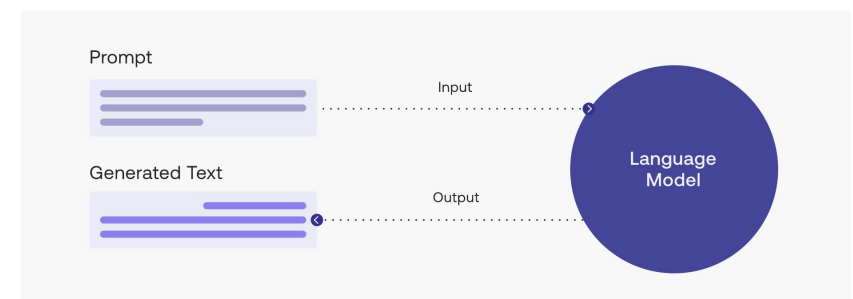
\includegraphics[width=\linewidth,keepaspectratio]{promptengg2}

{\tiny (Ref: Cohere https://docs.cohere.ai/docs/prompt-engineering)}

\end{center}				
			
			

\end{frame}



%%%%%%%%%%%%%%%%%%%%%%%%%%%%%%%%%%%%%%%%%%%%%%%%%%%%%%%%%%%
\begin{frame}[fragile]\frametitle{What is a Language Models?}

\begin{itemize}
\item While typing SMS, have you seen it suggests next word?
\item While typing email, have you seen next few words are suggested?
\item How does it suggest? (suggestions are not random, right?)
\item In the past, for ``Lets go for a \ldots', if you have typed 'coffee' 15 times, 'movie' say 4 times, then it learns that. Machine/Statistical Learning.
\item Next time, when you type ``Lets go for a '', what will be suggested? why?
\item This is called Language Model. Predicting the next word. When done continuously, one after other, it spits sentence, called Generative Model.
\end{itemize}	

\begin{center}
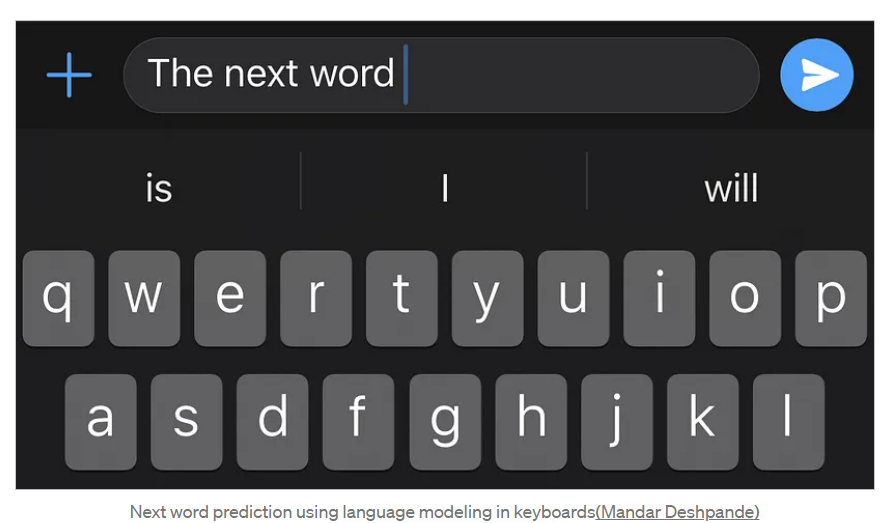
\includegraphics[width=0.6\linewidth,keepaspectratio]{chatgpt34}
\end{center}		

\end{frame}

%%%%%%%%%%%%%%%%%%%%%%%%%%%%%%%%%%%%%%%%%%%%%%%%%%%%%%%%%%%
\begin{frame}[fragile]\frametitle{Evolution of Language Models}

Language Models can be statistical (frequency based) or Machine/Deep Learning (supervised) based. Simple to complex.

\begin{center}
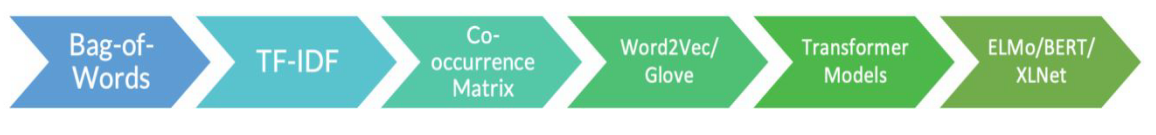
\includegraphics[width=\linewidth,keepaspectratio]{chatgpt30}
\end{center}				
{\tiny (Ref: Analytics Vidhya https://editor.analyticsvidhya.com/uploads/59483evolution\_of\_NLP.png)}

\end{frame}

%%%%%%%%%%%%%%%%%%%%%%%%%%%%%%%%%%%%%%%%%%%%%%%%%%%%%%%%%%%
\begin{frame}[fragile]\frametitle{Large Language Models - Comparison}

\begin{center}
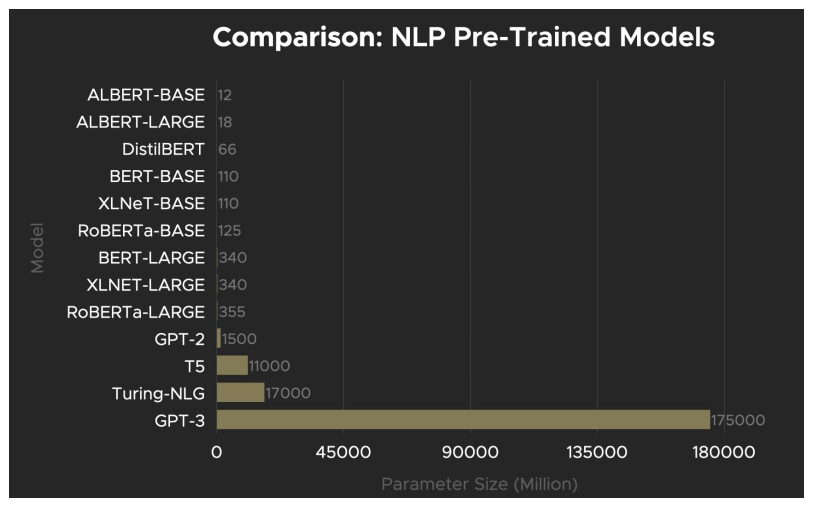
\includegraphics[width=\linewidth,keepaspectratio]{chatgpt31}
\end{center}				
{\tiny (Ref: Deus.ai https://www.deus.ai/post/gpt-3-what-is-all-the-excitement-about)}

\end{frame}

%%%%%%%%%%%%%%%%%%%%%%%%%%%%%%%%%%%%%%%%%%%%%%%%%%%%%%%%%%%
\begin{frame}[fragile]\frametitle{What is Prompt Engineering?}

How to talk to AI to get it to do what you want


\begin{center}
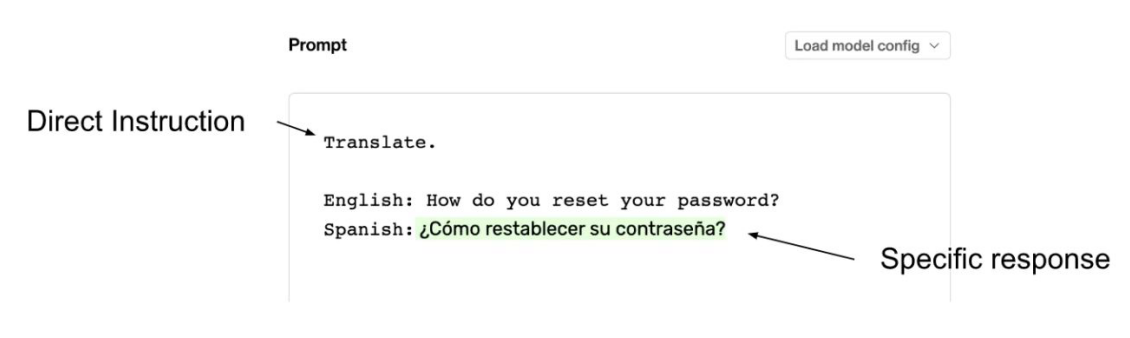
\includegraphics[width=\linewidth,keepaspectratio]{promptengg3}

{\tiny (Ref: Human Loop https://humanloop.com/blog/prompt-engineering-101)}

\end{center}				
			

\end{frame}

%%%%%%%%%%%%%%%%%%%%%%%%%%%%%%%%%%%%%%%%%%%%%%%%%%%%%%%%%%%
\begin{frame}[fragile]\frametitle{What is Prompt Engineering?}

But need to tell, for sure, else, nothing


\begin{center}
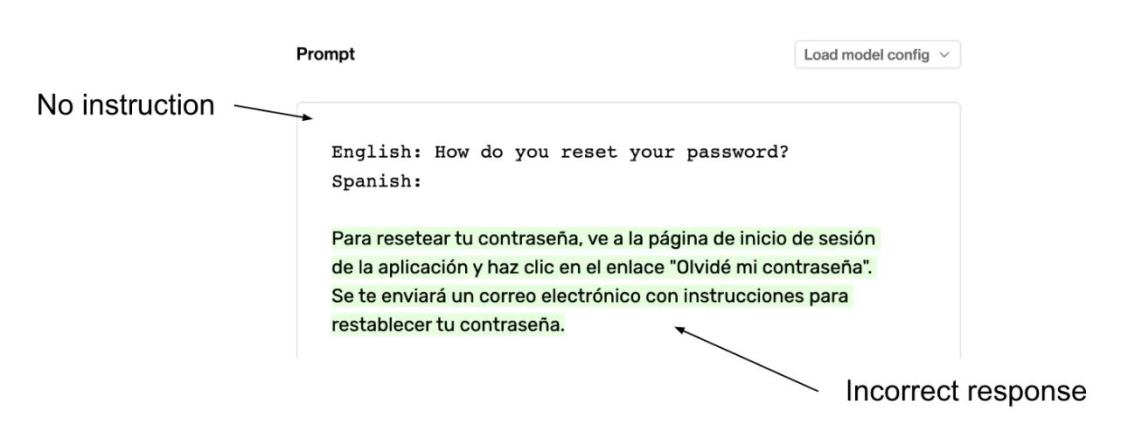
\includegraphics[width=\linewidth,keepaspectratio]{promptengg4}

{\tiny (Ref: Human Loop https://humanloop.com/blog/prompt-engineering-101)}

\end{center}				

\end{frame}


%%%%%%%%%%%%%%%%%%%%%%%%%%%%%%%%%%%%%%%%%%%%%%%%%%%%%%%%%%%
\begin{frame}[fragile]\frametitle{What is Prompt Engineering?}

\begin{itemize}
\item For prompt \lstinline|What is 1,000,000 * 9,000?| GPT-3 (text-davinci-002) (an AI) sometimes answers 9,000,000 (incorrect). This is where prompt engineering comes in.
\item If, instead of asking What is \lstinline|1,000,000 * 9,000?|, we ask \lstinline|What is 1,000,000 * 9,000? Make sure to put the right amount of zeros, even if there are many:|, GPT-3 will answer 9,000,000,000 (correct). 
\item Why is this the case? Why is the additional specification of the number of zeros necessary for the AI to get the right answer? How can we create prompts that yield optimal results on our task? 			
\item That's Prompt Engineering.
\end{itemize}

{\tiny (Ref: https://learnprompting.org/docs/basics/prompting)}
\end{frame}
